\documentclass[11pt, a4paper]{toptesi}

\usepackage[utf8]{inputenc} %utf8
\usepackage[english]{babel}
\usepackage[T1]{fontenc}
\usepackage{blindtext}
\usepackage{graphicx,wrapfig}
\usepackage{booktabs}
\usepackage{lmodern}
\usepackage{varioref}
\usepackage{url}
\usepackage{array}
\usepackage{verbatim} 
\usepackage{subfig}
\usepackage{tabularx}
\usepackage{amsmath}
\usepackage{amsfonts}
\usepackage{float}
\usepackage{amssymb}
\usepackage{multicol}
\usepackage{multirow}
\usepackage{listings}
\usepackage{algorithm}
\usepackage{algorithmic}
\usepackage{amsmath}
\usepackage{hyperref}
\usepackage{minted}
\usepackage{fancyhdr}
\frenchspacing
\pagestyle{fancy}
\begin{document}

\paragraph{Laboratory report (Camera calibration and rectification) - Luca Dolci
    1234008}
The flow control of the program follows the standard worflow of the camera
calibration and image rectification process:
\begin{enumerate} \setcounter{enumi}{-1}
    \item \underline{Input parsing and parameters setting:} the program computes
        the calibration using some checkerboard photos. The first thing that
        the program does is to ask the user the directory under which the
        photos are saved (in png format). After this, the program ask again the
        user to input some checkerboard proprieties: the number of (inner!) rows
        and columns of the checkerboard and the size of the checkerboard's
        squares (in
        meters). 
        It it possible to set some flags as well as the monitor's size as
        command line arguments in this format:
        \begin{minted}{R}
        ./lab2 debug screen_height screen_width
        \end{minted}
        where \mintinline{R}{debug} is a 0-1 flag for visualization of the checkerboard
        images during corners detection, \mintinline{R}{screen_height} and 
        \mintinline{R}{screen_width} are the dimensions of your monitor 
        (to adapt the visualization). 
    
    \item \underline{Checkerboard corners detection}: the corners detection is
        performed by the \\
        \mintinline{R}{findChessboardCorners()} function. Then,
        if enough corners are detected, the detection is refined using the
        \mintinline{R}{cornerSubPix()} fucntion. The coners detection can fail
        if some corners are not present or if the checkerboard
        is physically far from the camera (this also depends on the photo's
        spatial resolution). In this step, apart from the corners 2D points, also
        the 3D points are computed using the
        \mintinline{R}{find3Dcorners()}and saved. If debug mode is activated, the result of a detection is the seguent:
        \begin{center}
        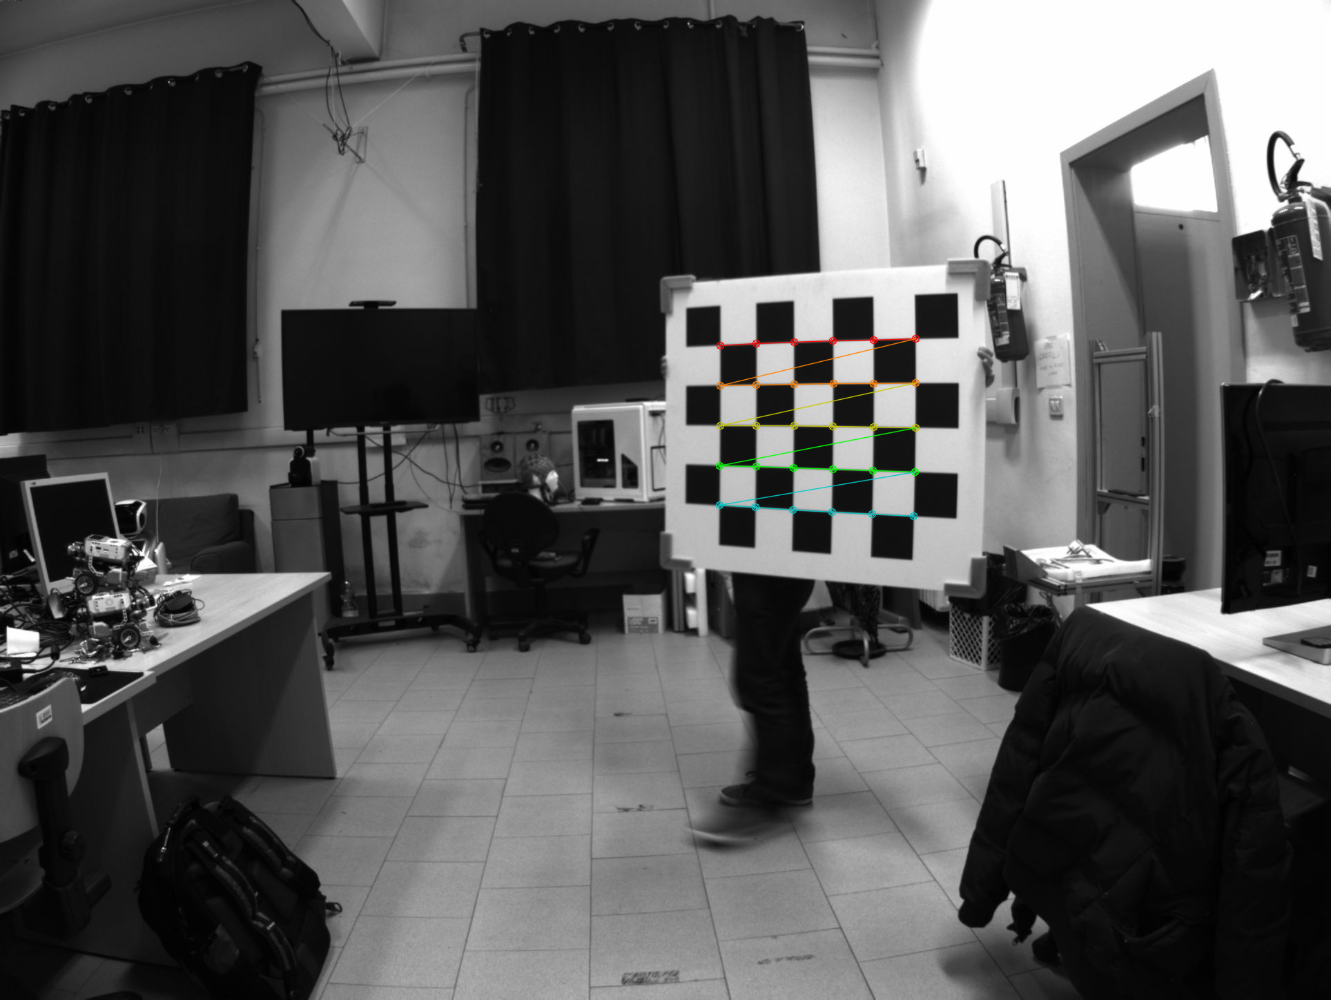
\includegraphics[width=0.6\textwidth]{./checkerboard_corner_detection.png}
        \end{center}

    \item \underline{Camera calibration}: the calibration is performed by the
        \mintinline{R}{calibrateCamera()} function that, given the points
        detected in step 1, produces the camera
        matrix and the radial and tangential distortion parameters.

    \item \underline{Reprojection error computation}: this can be done by
        projecting the 3D point computed in step 1 with the camera matrix
        computed in step 2 (using the \mintinline{R}{projectPoint()}
        function). The reprojection error for each photo is computed as the sum
        of the euclidean distances from corners and projected points. Then the
        best and worse photos (in term of reprojection error) are find and
        their name are printed.

    \item \underline{Rectification}: given the camera matrix and the distortion
        coefficents, two maps are computed using the
        \mintinline{R}{initUndistortRectifyMap()} function. Also, a new camera
        matrix is computed but it is not necessary because only the two maps are
        needed by the \mintinline{R}{remap()} function in order to perform the
        rectification. The final result is the seguent:
        
        \begin{center}
            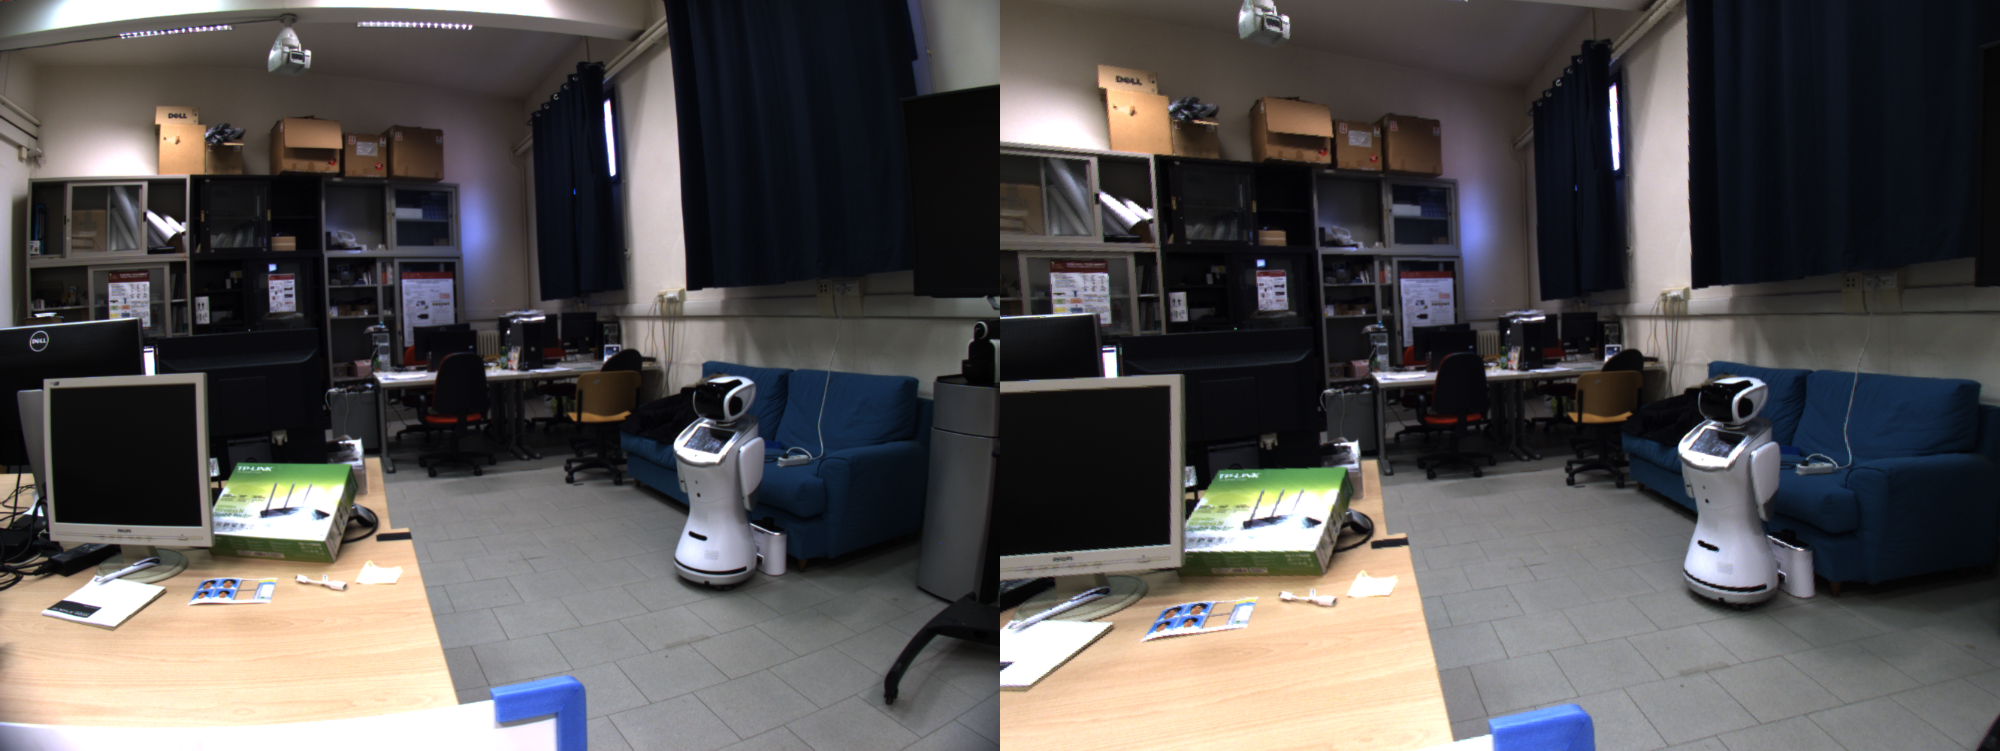
\includegraphics[width=0.9\textwidth]{./rectification.png}
        \end{center}
\end{enumerate}



\end{document}
